\section{Resultados}

\subsection{Comparación de técnicas para promediar datos} \label{resultados:comparacionDeMetricas}

\begin{figure}[h!]
 \centering
 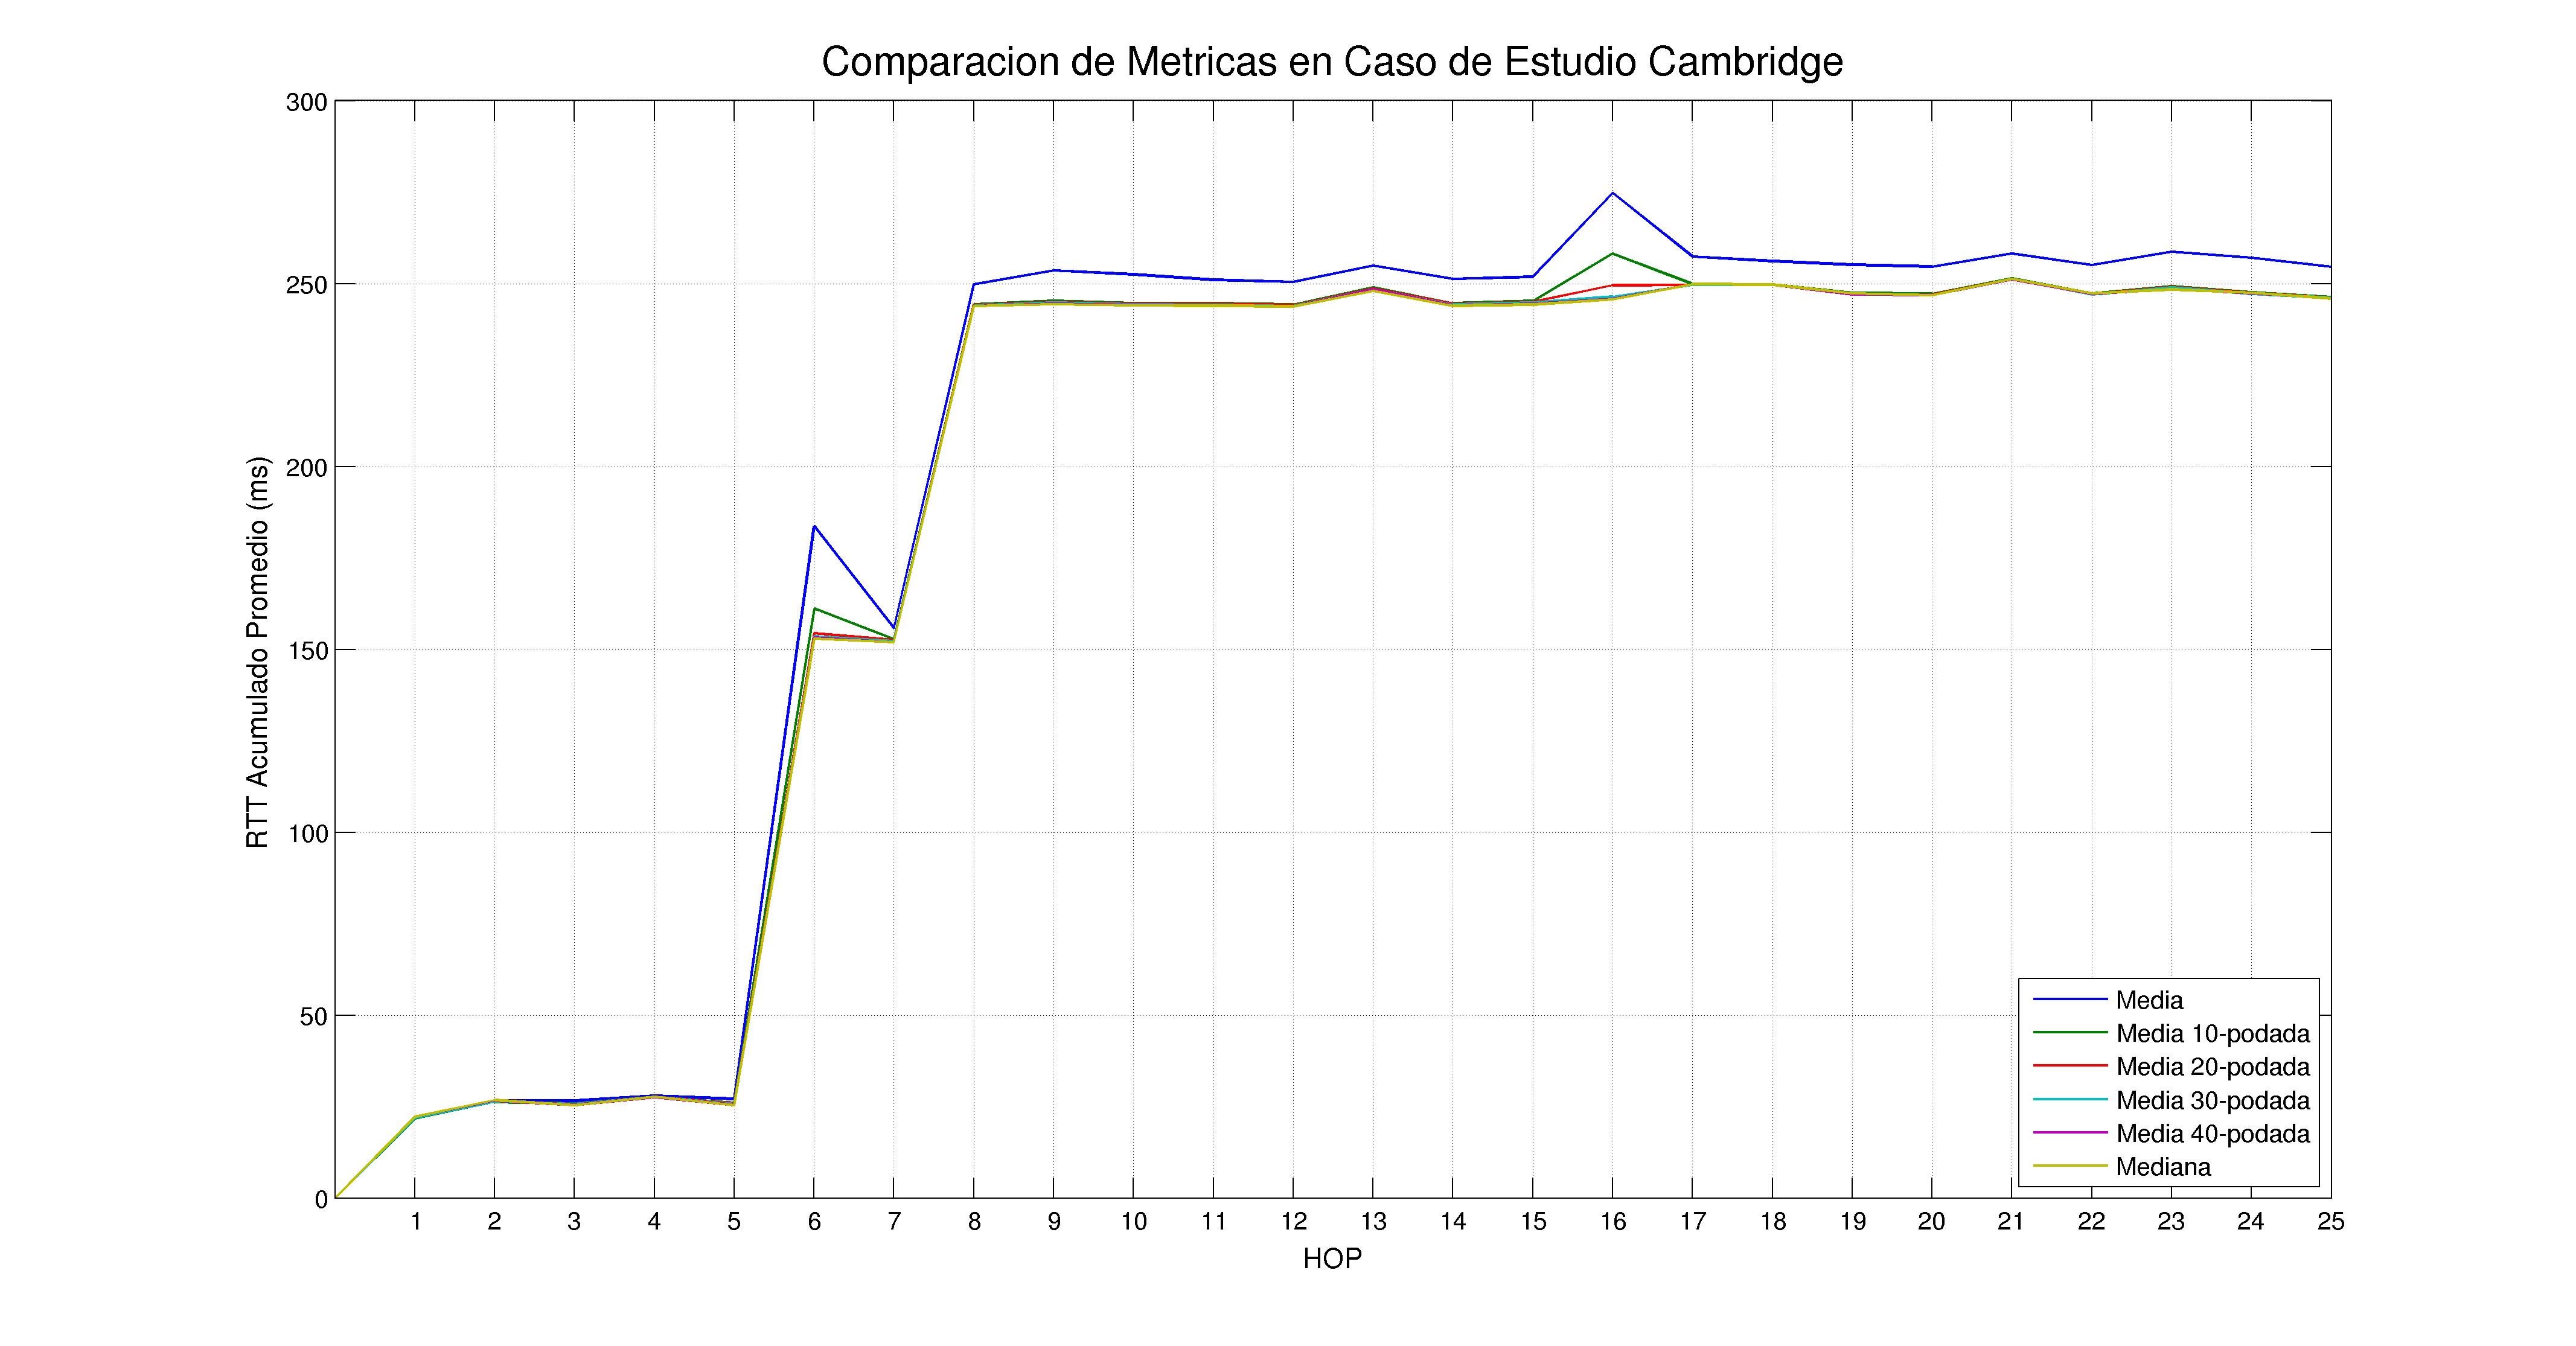
\includegraphics[width=\textwidth]{../resultados/comparacion-metricas-cambridge.png}
 \caption{Comparación de las distintas técnicas para promediar el RTT acumulado, en el caso de estudio de la universidad de Cambridge.}
\end{figure}

\begin{figure}[h!]
 \centering
 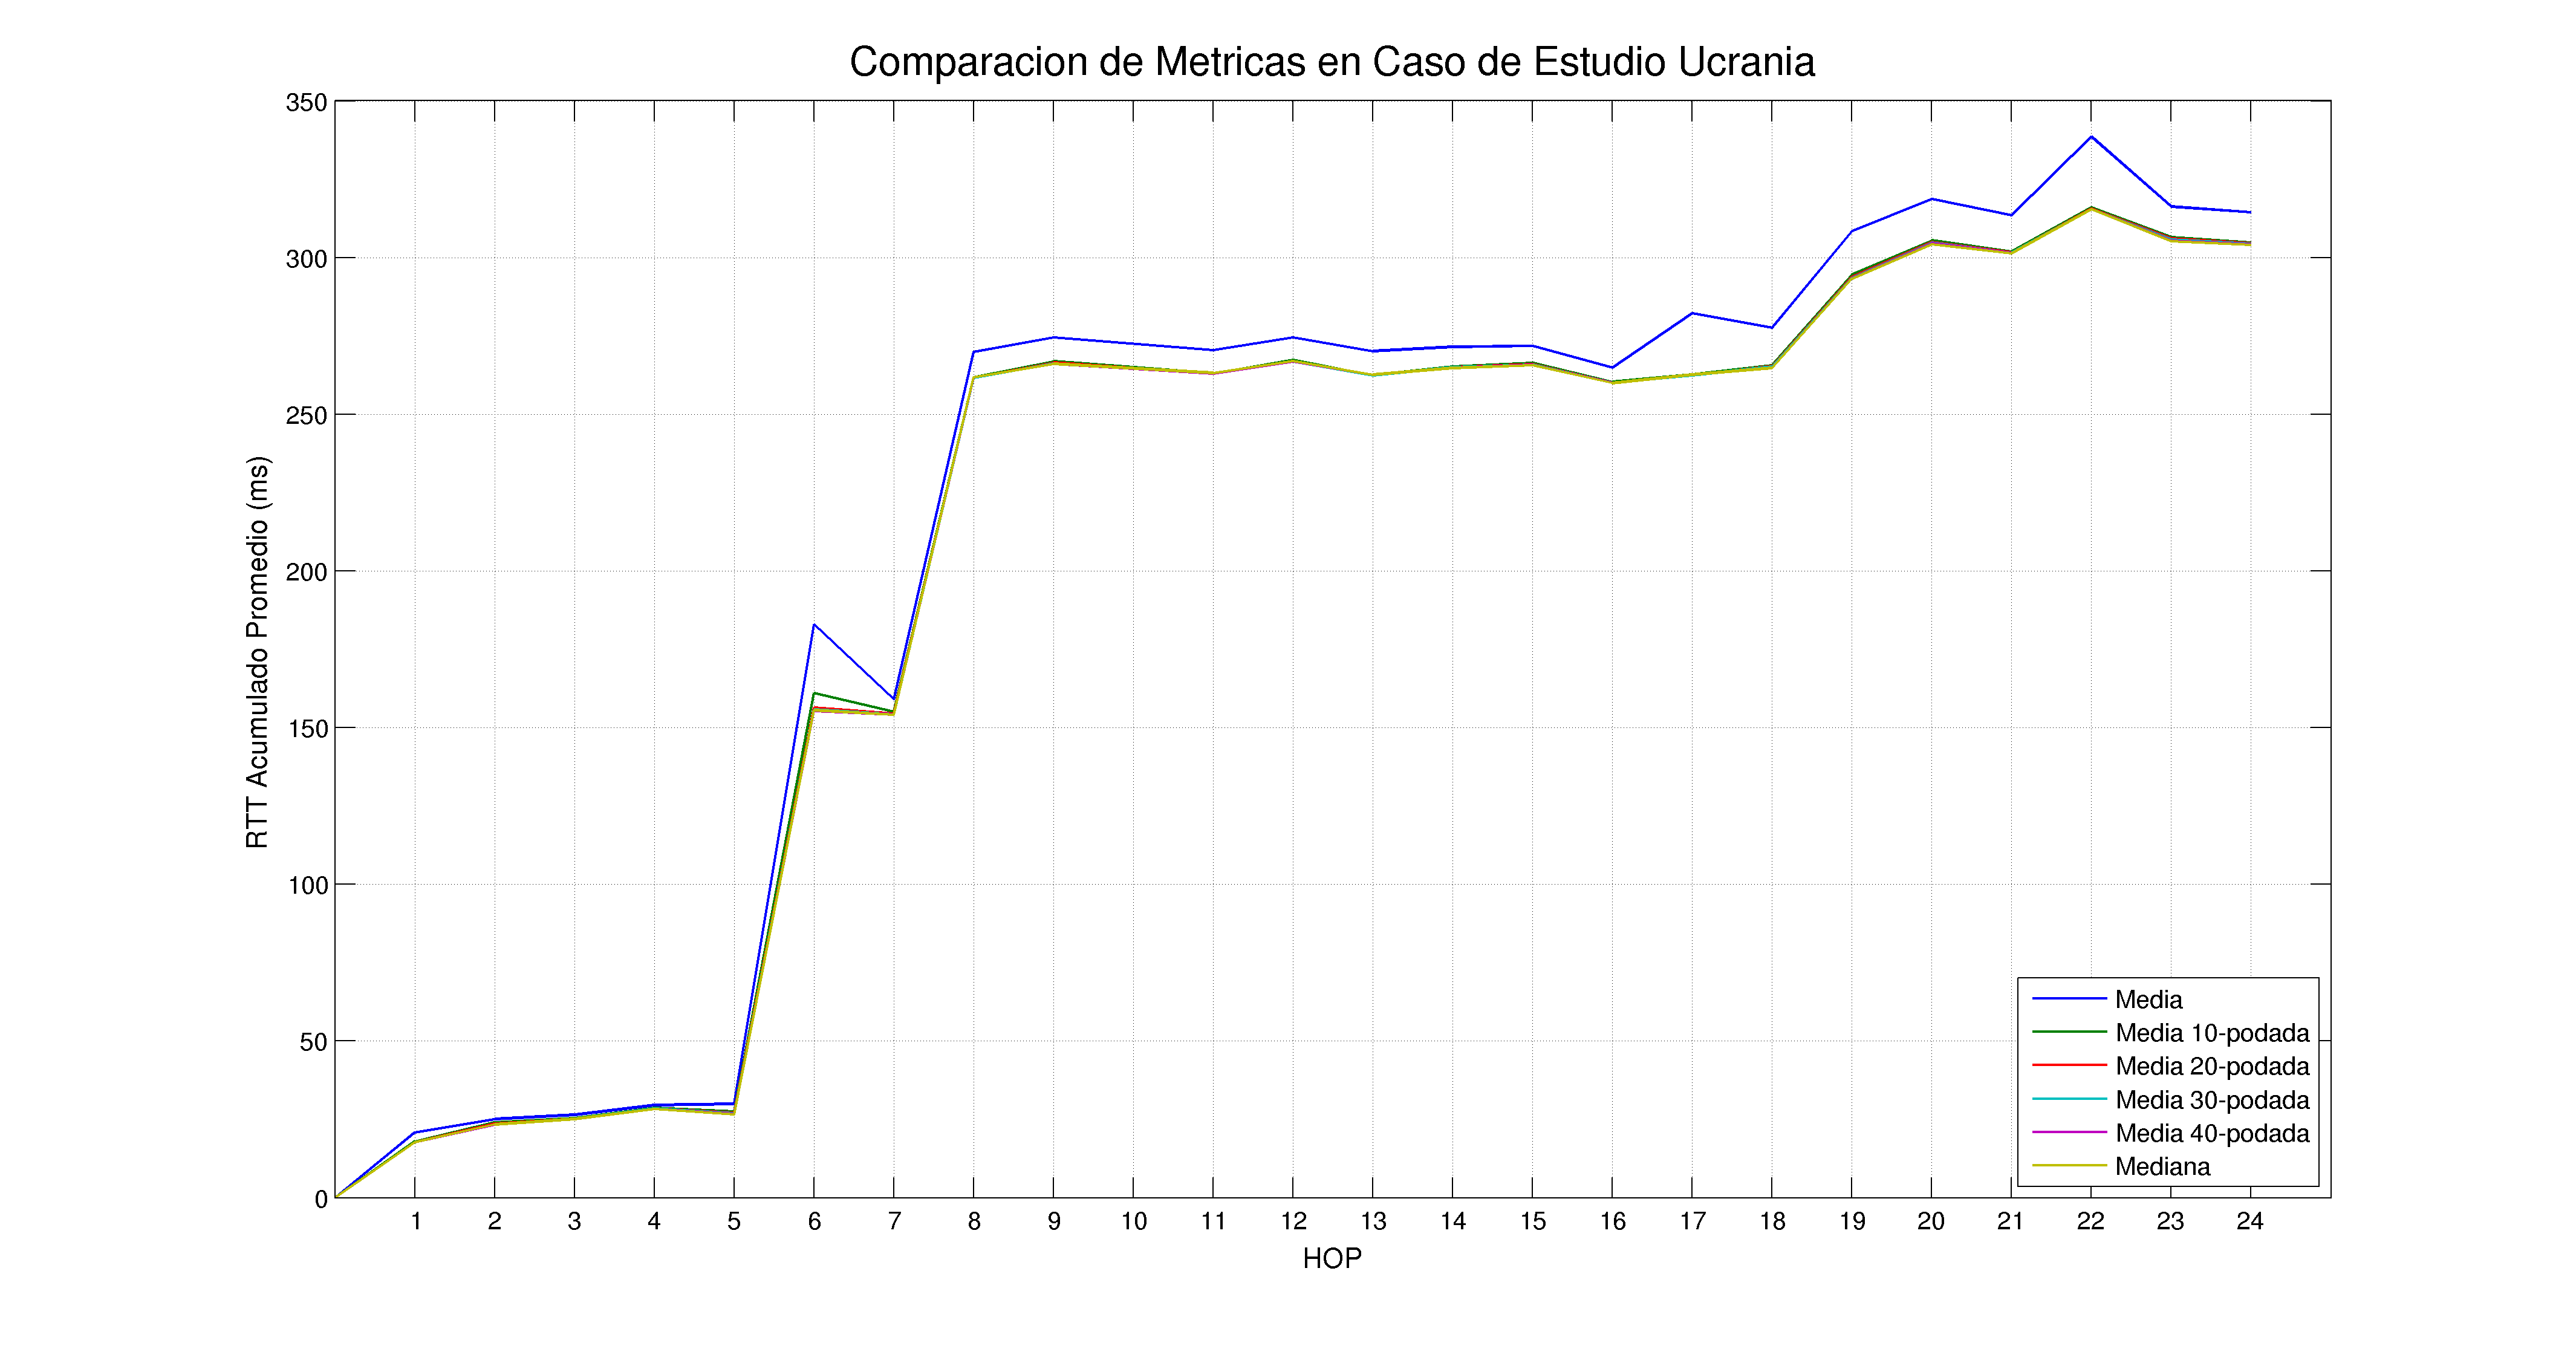
\includegraphics[width=\textwidth]{../resultados/comparacion-metricas-ucrania.png}
 \caption{Comparación de las distintas técnicas para promediar el RTT acumulado, en el caso de estudio de la universidad de Ucrania.}
\end{figure}

\newpage

\begin{figure}[h!]
 \centering
 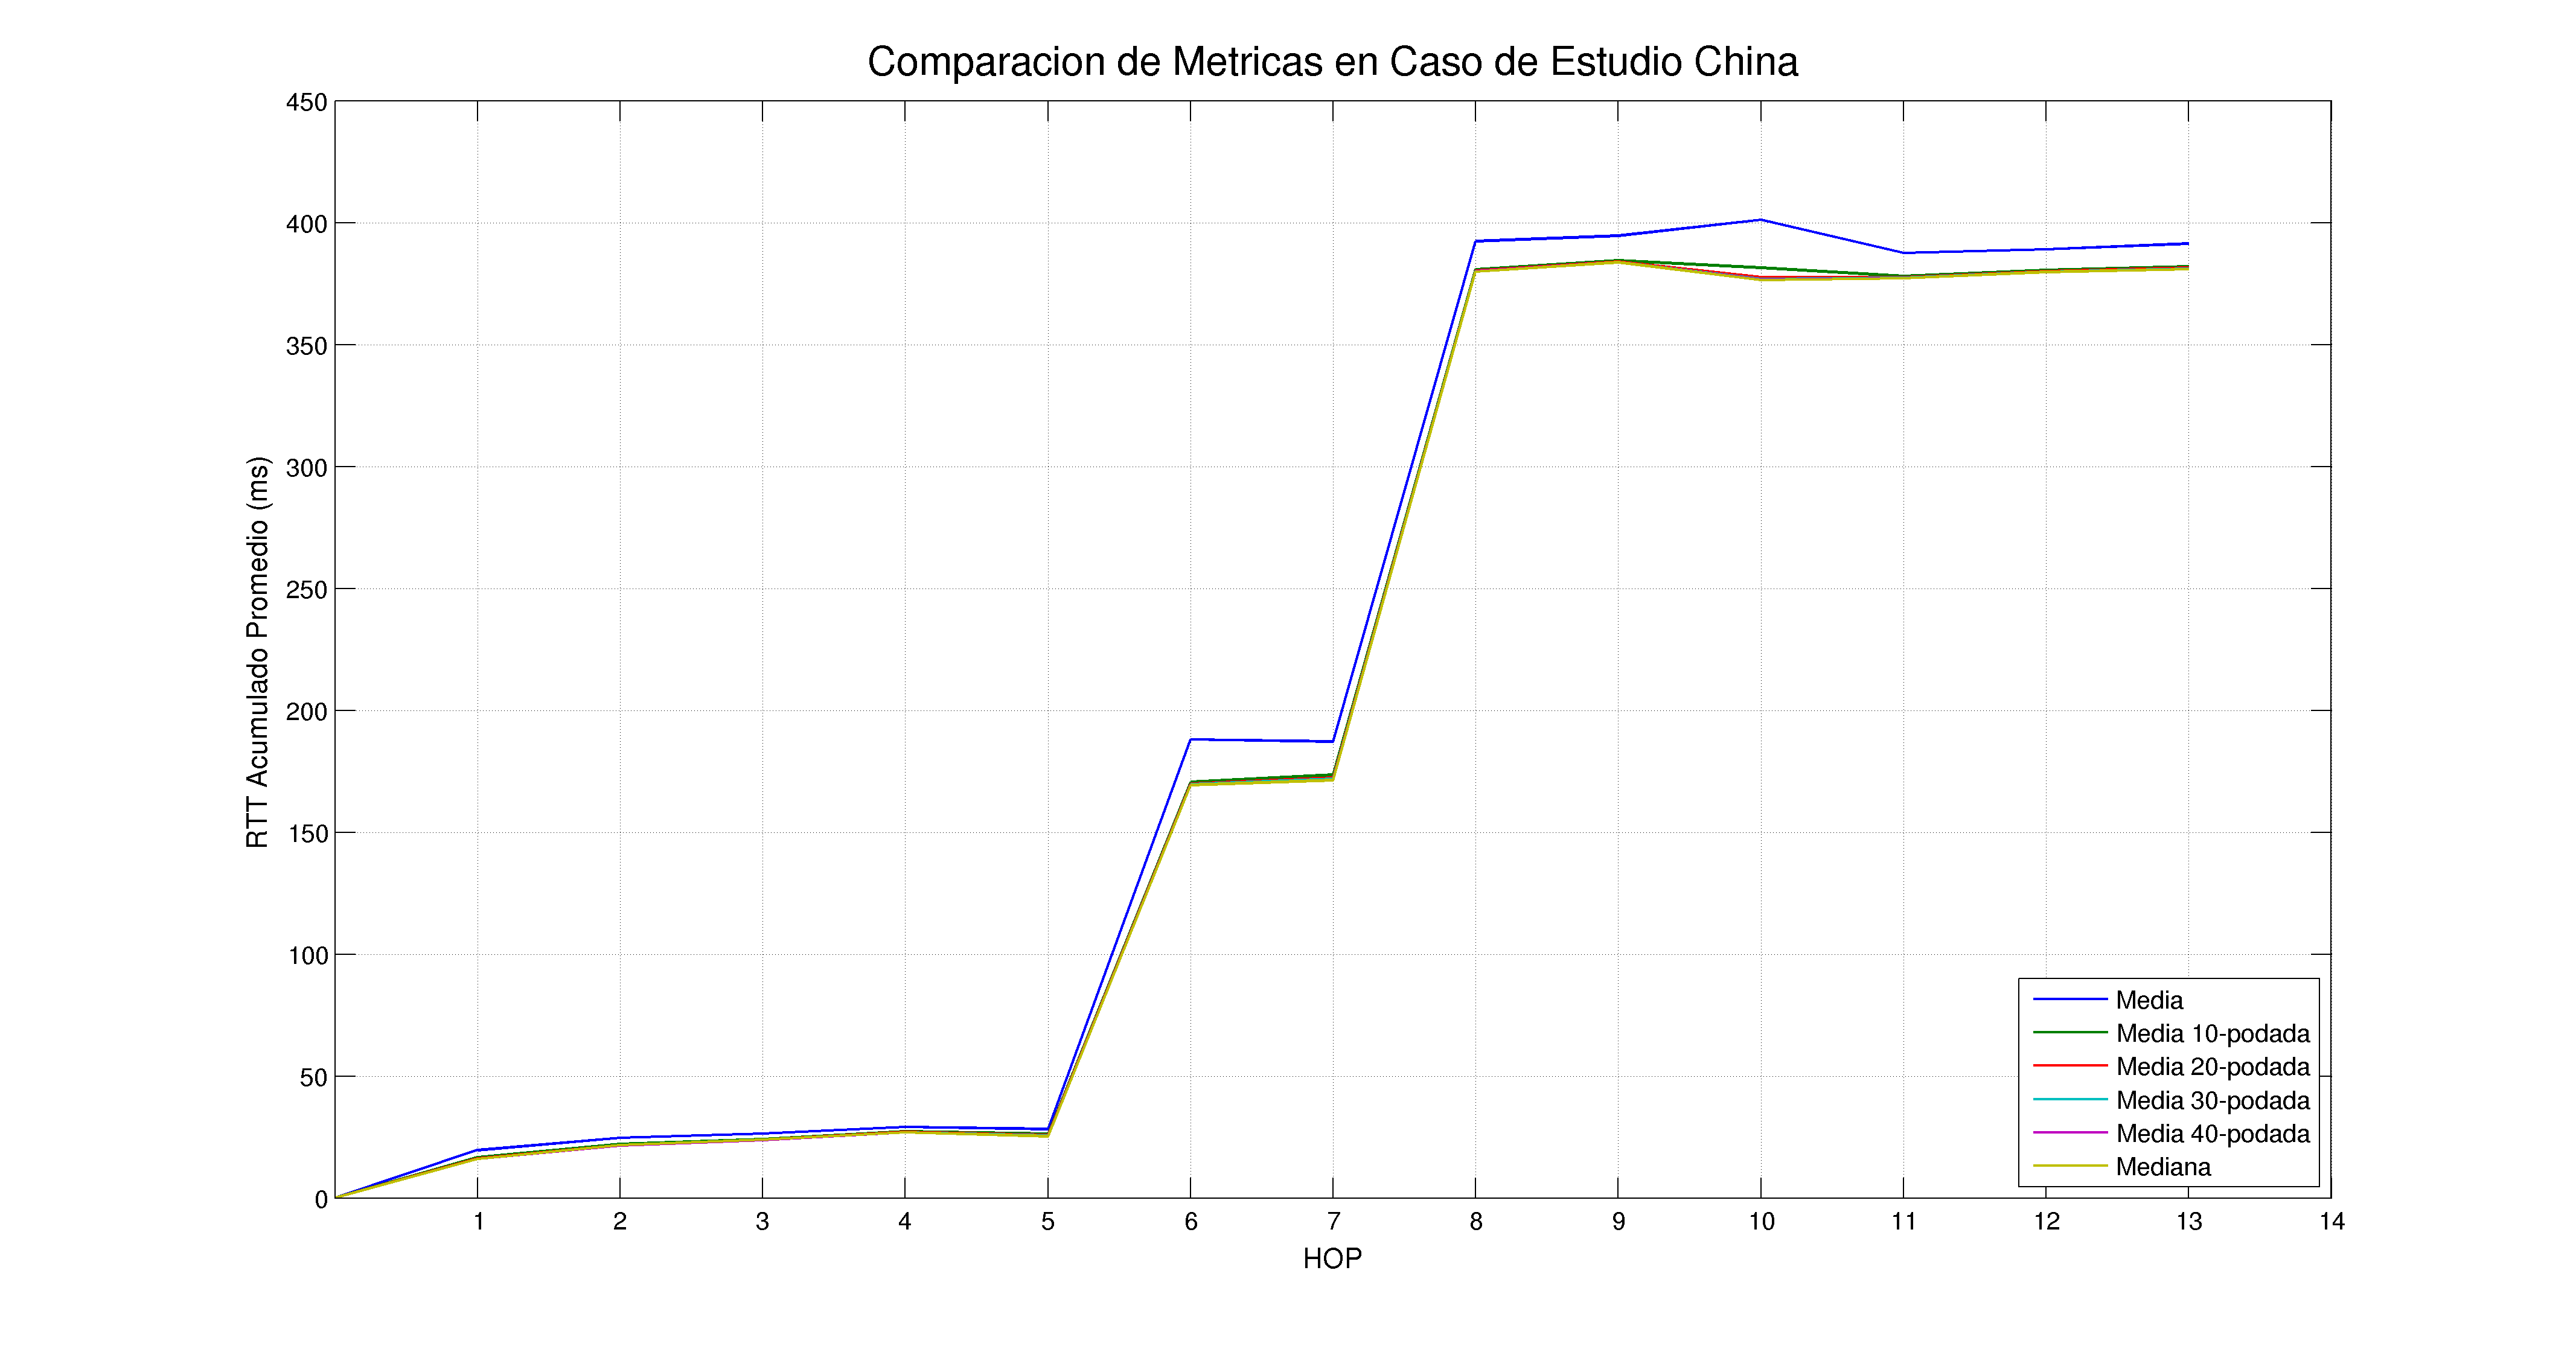
\includegraphics[width=\textwidth]{../resultados/comparacion-metricas-china.png}
 \caption{Comparación de las distintas técnicas para promediar el RTT acumulado, en el caso de estudio de la universidad de China.}
\end{figure}

\newpage

\subsection{Caso de Estudio: Universidad de Cambridge} \label{resultados:cambridge}
\subsubsection{Determinación de Rutas y RTTs de cada salto}
%% Aca decir que se encontró una sola ruta y ponemos directamente la tablita (ttl,ip,icmp,rttAcum,probabilidad,rtt_1_i,rtt_2_i)
%% rtt_1_i vs rtt_2_i

\begin{table}[h!]
  \footnotesize
  \centering
  \begin{tabular}{| r | r | c | r | r | r | r |}
  \hline
  \multicolumn{7}{|c|}{\bf Ruta Más Probable: Cambridge}\\
  \hline\hline
  {\bf\footnotesize TTL} & \multicolumn{1}{|c|}{\bf\footnotesize IP} & \multicolumn{1}{|c|}{\bf\footnotesize ICMP} & {\bf\footnotesize $P(IP|TTL)$} & {\bf\footnotesize $RTT^{acum}_i$ (ms)} & {\bf\footnotesize 1. $RTT_i$ (ms)}& {\bf\footnotesize 2. $RTT_i$ (ms)}\\
  \hline
  \hline
  %%%% TABLA QUE PRODUCE calcular.py :
  \input{../resultados/tabla-cambridge.tab}
  \end{tabular}
  \caption{El camino más utilizado para llegar a Cambridge. Los encabezados utilizan la notación presentada en las secciones \ref{desarrollo:rutas}
  y \ref{desarrollo:rttPorSalto}.}
\end{table}
%% De esta tabla hay que decir: porque rtts acumulados no son estrictamente crecientes, cual es mejor RTT_i segun cual nos da mas informacion,
%% que la ruta es unica porque todas las ips dieron con proba=1, los RTT=0 se corresponden con ips dentro de un mismo sistema autonomo?

\subsubsection{RTTs acumulados y ZRTTs}

\begin{figure}[h!]
 \centering
 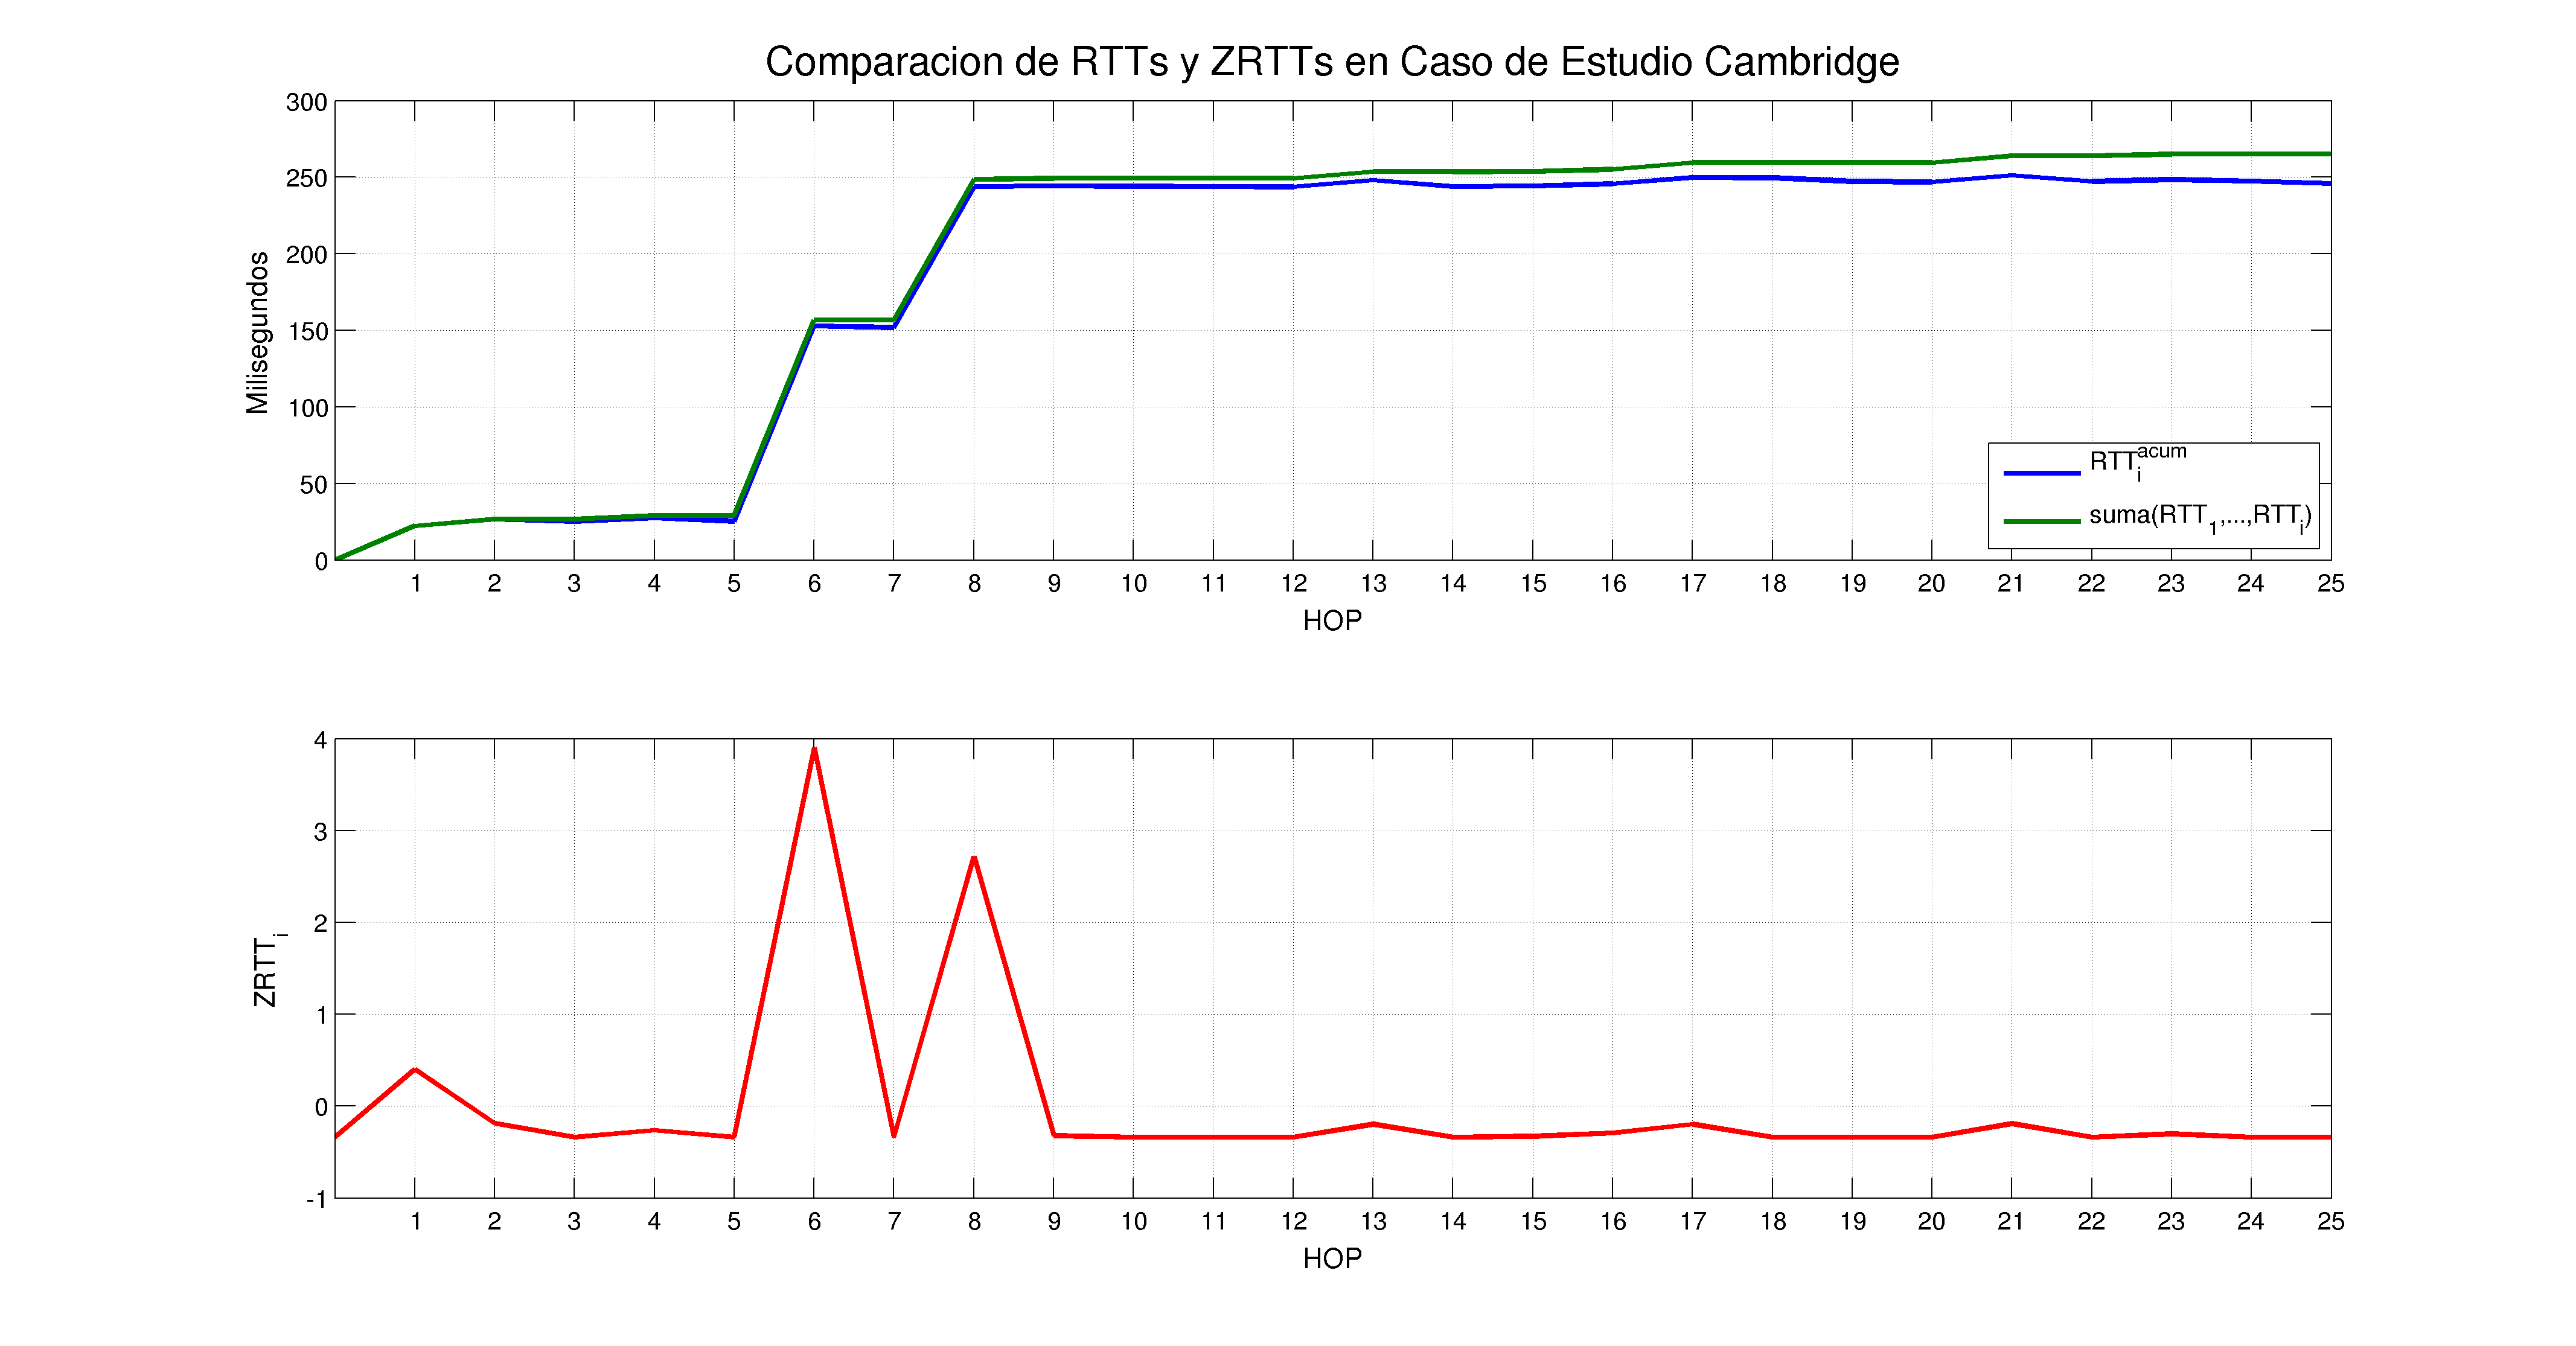
\includegraphics[width=\textwidth]{../resultados/comparacion-zrtts-cambridge.png}
 \caption{Comparación de $RTT^{acum}_i$ con $\sum_{k=1}^{i}RTT_k$ y con $ZRTT_i$.}
 \label{resultados:cambridge:zrtt}
\end{figure}

\newpage

\subsubsection{Geolocalización}

% \begin{figure}[h!]
%  \centering
%  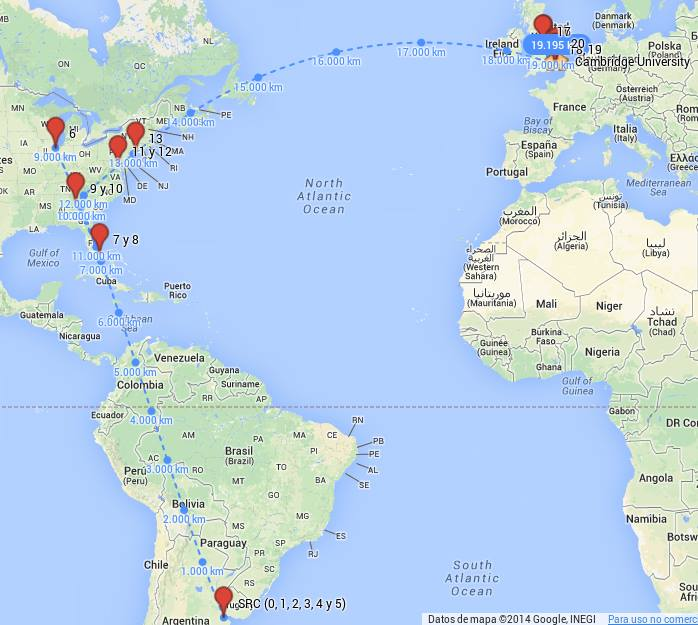
\includegraphics[width=0.5\textwidth]{../resultados/mapa-cambridge-1.jpg}
%  
%  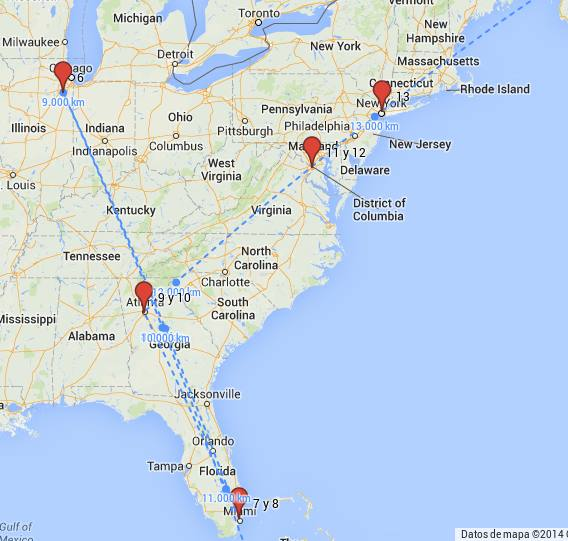
\includegraphics[width=0.45\textwidth]{../resultados/mapa-cambridge-2.jpg}
%  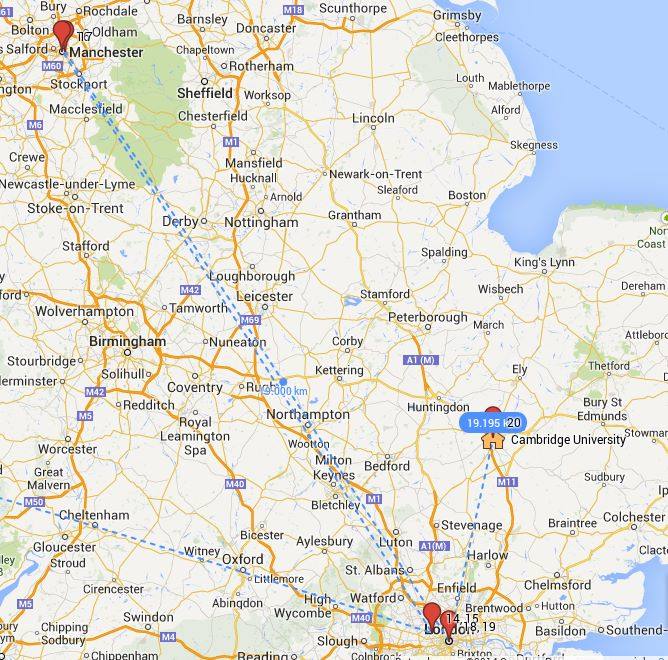
\includegraphics[width=0.45\textwidth]{../resultados/mapa-cambridge-3.jpg}
% 
%  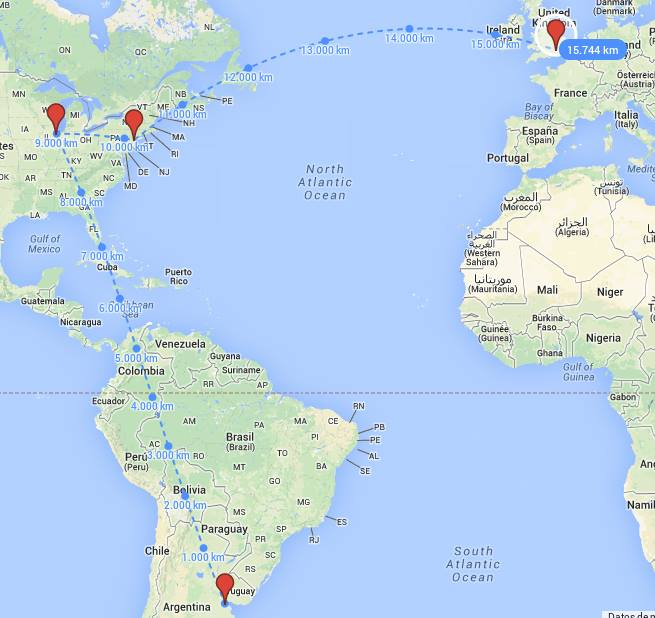
\includegraphics[width=0.5\textwidth]{../resultados/mapa-cambridge-4.jpg}
%  \caption{Mapa}
% \end{figure}
% %% Mapa geolocalizando la ruta
% %% distancias vs rtts, acertamos al enlace submarino con los zscores?
% 
% \newpage

\begin{table}[h!]
  \centering
  \scriptsize
  \begin{adjustwidth}{-1cm}{}
    \begin{tabular}{| r | r | c | c | c |}
    \hline
    \multicolumn{5}{|c|}{\bf Geolocalización: Cambridge}\\
    \hline\hline
    {\bf TTL} & \multicolumn{1}{|c|}{\bf IP} & \multicolumn{1}{|c|}{\bf DNS} & {\bf Ubicación} & {\bf Lat,Lon}\\
    \hline
    \hline
    %%%% TABLA QUE PRODUCE calcular.py :
    \input{../resultados/geoloc-cambridge.tab}
    \end{tabular}
  \end{adjustwidth}
  \caption{\footnotesize Tabla de información de geolocalización del camino más probable para el caso de estudio Cambridge. Observar las celdas resaltadas de arriba hacia abajo: (1) indica que comenzamos en Argentina. (2) dice ``{\tt crossing-argentina}'' lo cual indica que seguimos en Argentina o  cerca. (3) dice ``{\tt ar1.MIA2}'' mientras que las dos anteriores decían ``{\tt ar3.eze1}'' indicando que algo cambió, la red también cambió (ver la IP) y además este salto corresponde al de mayor RTT. (4) El salto para TTL=8 corresponde al segundo salto de mayor RTT, sin embargo de los datos de geolocalización
  no podemos inferir que sea un enlace submarino. (5) Recien en el salto 14 aparece en la DNS la palabra ``{\tt London}'' haciendo referencia
  a Inglaterra (el salto anterior aún decía Estados Unidos en la DNS). (6) Recién en el salto 17 aparece la geolocalización en United Kingdom.}
\end{table}

\begin{figure}[h!]
 \centering
 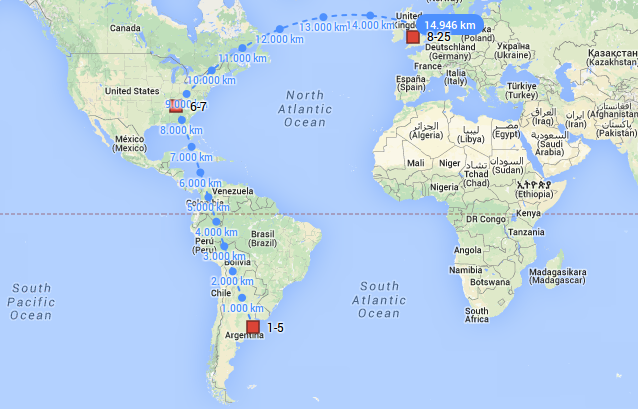
\includegraphics[width=\textwidth, trim = 0 50 0 0, clip]{../resultados/mapa-cambridge.png}
 \caption{Mapa generado utilizando los datos de la tabla anterior y los valores de $RRT_i$ empíricos.}
\end{figure}

\newpage

\subsection{Caso de Estudio: Universidad de Ucrania} \label{resultados:ucrania}

\subsubsection{Determinación de Rutas y RTTs de cada salto}
%% Aca decir que se encontró una sola ruta y ponemos directamente la tablita (ttl,ip,icmp,rttAcum,probabilidad,rtt_1_i,rtt_2_i)
%% rtt_1_i vs rtt_2_i

% \begin{table}[h!]
%   \centering
%   \footnotesize
%   \begin{tabular}{| r || r | c | r || r | c | r || r | c | r |}
%   \hline
%   \multicolumn{10}{|c|}{\bf Rutas Más Probables}\\
%   \hline\hline
%   {\bf\footnotesize TTL} & \multicolumn{1}{|c|}{\bf\footnotesize IP1} & \multicolumn{1}{|c|}{\bf\footnotesize ICMP1} & {\bf\footnotesize P1}  & \multicolumn{1}{|c|}{\bf\footnotesize IP2} & \multicolumn{1}{|c|}{\bf\footnotesize ICMP2} & {\bf\footnotesize P2} & \multicolumn{1}{|c|}{\bf\footnotesize IP3} & \multicolumn{1}{|c|}{\bf\footnotesize ICMP3} & {\bf\footnotesize P3}\\
%   \hline
%   \hline
%   %%%% TABLA QUE PRODUCE calcular.py :
%   \input{../resultados/kiev_caminos_latex.txt}
%   \end{tabular}
%   \caption{Los caminos más utilizado para llegar a Ucrania. Los encabezados utilizan la notación presentada en las secciones \ref{desarrollo:rutas}
%   y \ref{desarrollo:rttPorSalto}.}
% \end{table}

\begin{table}[h!]
  \centering
  \footnotesize
  \begin{tabular}{| r || r | c | r || r | c | r |}
  \hline
  \multicolumn{7}{|c|}{\bf Rutas Encontradas: Ucrania}\\
  \hline\hline
  {\bf\footnotesize TTL} & \multicolumn{1}{|c|}{\bf\footnotesize IP1} & \multicolumn{1}{|c|}{\bf\footnotesize ICMP1} & {\bf\footnotesize P1}  & \multicolumn{1}{|c|}{\bf\footnotesize IP2} & \multicolumn{1}{|c|}{\bf\footnotesize ICMP2} & {\bf\footnotesize P2} \\
  \hline
  \hline
  %%%% TABLA QUE PRODUCE calcular.py :
  \input{../resultados/kiev_caminos_latex.txt}
  \end{tabular}
  \label{resultados:Ucrania:caminos}
  \caption{Las rutas encontradas para llegar a Ucrania. La numeración en los encabezados indica el número de ruta, ordenadas por probabilidad.}
\end{table}

\newpage
\begin{table}[h!]
  \centering
  \footnotesize
  \begin{tabular}{| r | r | c | r | r | r | r |}
  \hline
  \multicolumn{7}{|c|}{\bf Ruta Más Probable: Ucrania}\\
  \hline\hline
  {\bf\footnotesize TTL} & \multicolumn{1}{|c|}{\bf\footnotesize IP} & \multicolumn{1}{|c|}{\bf\footnotesize ICMP} & {\bf\footnotesize $P(IP|TTL)$} & {\bf\footnotesize $RTT^{acum}_i$ (ms)} & {\bf\footnotesize 1. $RTT_i$ (ms)}& {\bf\footnotesize 2. $RTT_i$ (ms)}\\
  \hline
  \hline
  %%%% TABLA QUE PRODUCE calcular.py :
  \input{../resultados/kiev_caminoMasProbable_latex.txt}
  \end{tabular}
  \label{resultados:Ucrania:camino}
  \caption{El camino más utilizado para llegar a Ucrania. Los encabezados utilizan la notación presentada en las secciones \ref{desarrollo:rutas}
  y \ref{desarrollo:rttPorSalto}.}
\end{table}
%% De esta tabla hay que decir: porque rtts acumulados no son estrictamente crecientes, cual es mejor RTT_i segun cual nos da mas informacion,
%% que la ruta es unica porque todas las ips dieron con proba=1, los RTT=0 se corresponden con ips dentro de un mismo sistema autonomo?


\subsubsection{RTTs acumulados y ZRTTs}

\begin{figure}[h!]
 \centering
 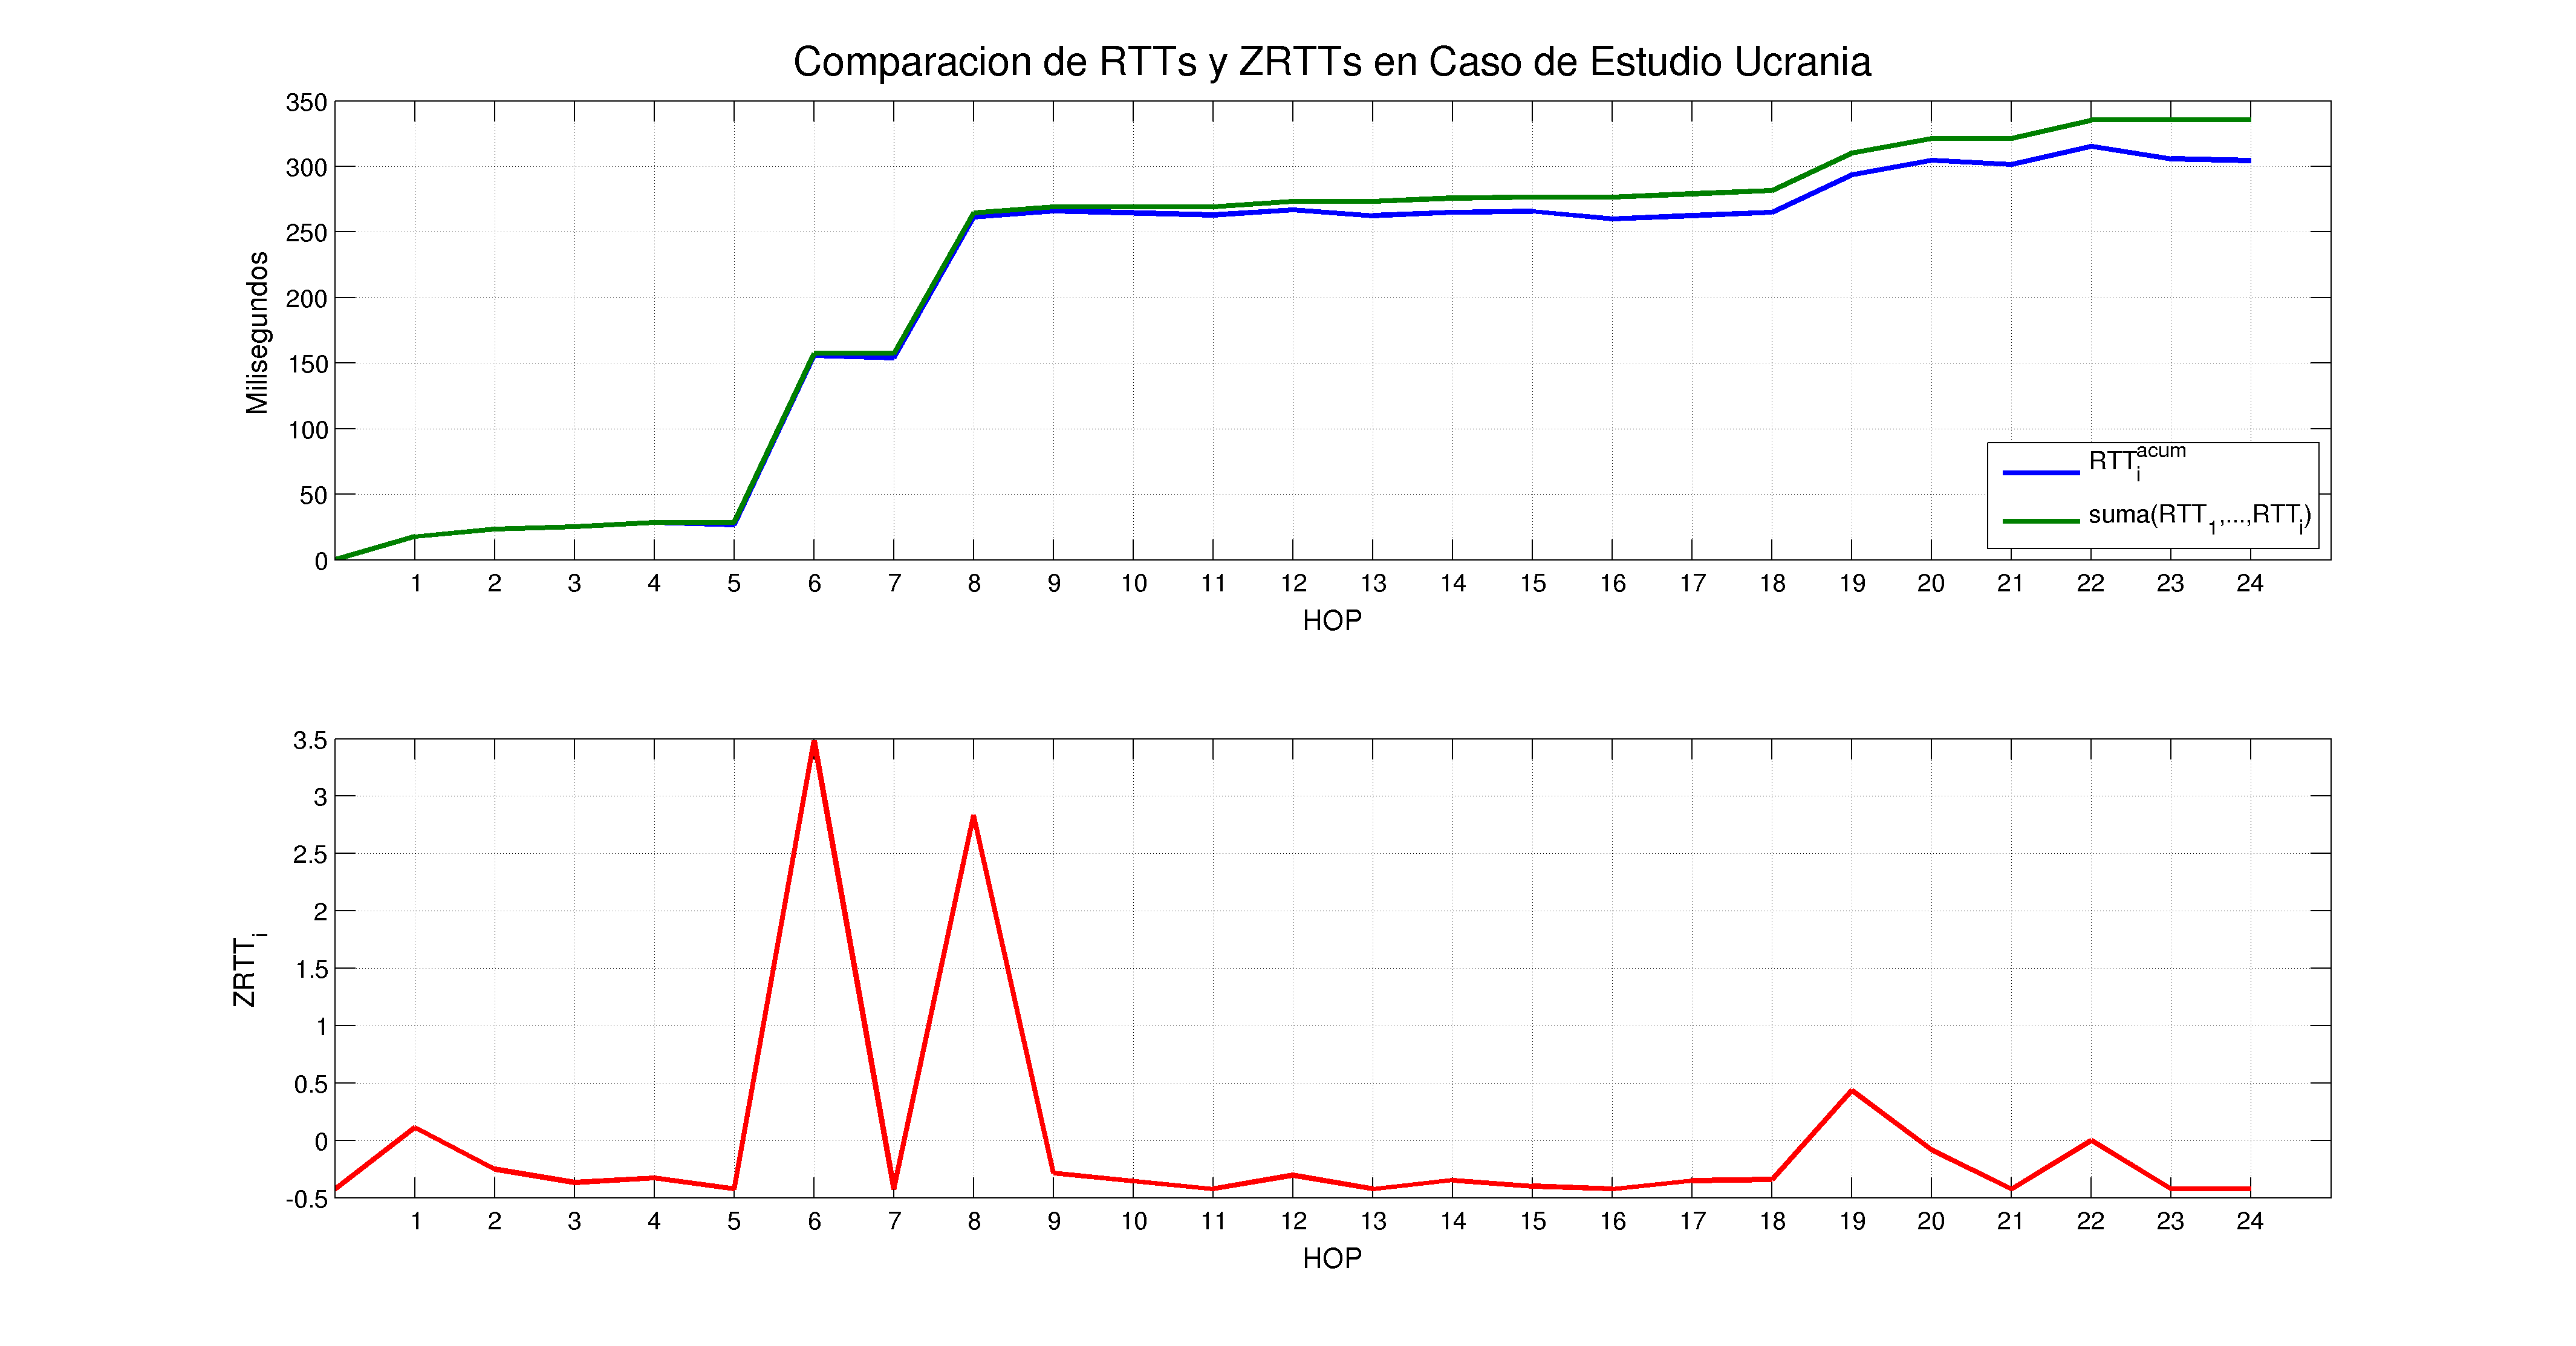
\includegraphics[width=\textwidth]{../resultados/comparacion-zrtts-ucrania.png}
 \caption{Comparación de $RTT^{acum}_i$ con $\sum_{k=1}^{i}RTT_k$ y con $ZRTT_i$.}
 \label{resultados:Ucrania:zrtt}
\end{figure}


\newpage
\subsubsection{Geolocalización}

\begin{table}[h!]
  \centering
  \scriptsize
  \begin{adjustwidth}{-0.6cm}{}
    \begin{tabular}{| r | r | c | c | c |}
    \hline
    \multicolumn{5}{|c|}{\bf Geolocalización: Ucrania}\\
    \hline\hline
    {\bf TTL} & \multicolumn{1}{c|}{\bf IP} & \multicolumn{1}{c|}{\bf DNS} & {\bf Ubicación} & {\bf Lat,Lon}\\
    \hline
    \hline
    %%%% TABLA QUE PRODUCE calcular.py :
    \input{../resultados/geoloc-ucrania.tab}
    \label{resultados:ucrania:geolocalizar}
    \end{tabular}
  \end{adjustwidth}
  \caption{\footnotesize Tabla de información de geolocalización del camino más probable para el caso de estudio Ucrania. Observar las celdas resaltadas de arriba hacia abajo: (1) indica que comenzamos en Argentina. (2) dice ``{\tt crossing-argentina}'' lo cual indica que seguimos en Argentina o  cerca. (3) dice ``{\tt ar1.MIA2}'' mientras que las dos anteriores decían ``{\tt ar3.eze1}'' indicando que algo cambió, la red también cambió (ver la IP) y además este salto corresponde al de mayor RTT. (4) El salto para TTL=8 corresponde al segundo salto de mayor RTT, sin embargo de los datos de geolocalización
  no podemos inferir que sea un enlace submarino. (5) Recien en el salto 14 aparece en la DNS la palabra ``{\tt Paris}'' haciendo referencia
  a Francia (el salto anterior aún decía Estados Unidos en la DNS). (6) En el salto 15 aparece en la DNS la palabra ``{\tt Frankfurt}'' haciendo
  referencia a Alemania (observar que aún la geolocalización indica Estados Unidos). (7) Por primera vez la geolocalización cambió de continente.
  (8) El salto 19 sobresale en cuanto al valor de RTT y además se corresponde con un salto intercontinental (no necesariamente submarino) de Europa
  a Asia, además observar que la DNS dice ``{\tt kiev}'' con lo cual podría ser que ya hemos llegado a Ucrania y la geolocalización es errónea. (9) La geolocalización indica Ucrania.}
\end{table}

\begin{figure}[h!]
 \centering
 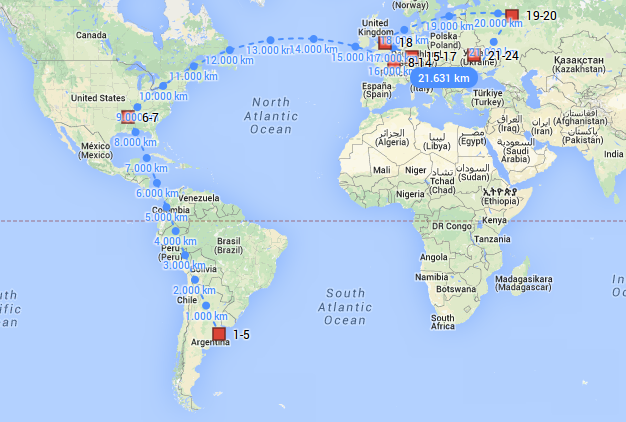
\includegraphics[width=\textwidth, trim = 0 60 0 0, clip]{../resultados/mapa-ucrania.png}
 \caption{Mapa generado utilizando los datos de la tabla anterior y los valores de $RRT_i$ empíricos.}
\end{figure}


\newpage
\subsection{Caso de Estudio: Universidad de China} \label{resultados:china}

\subsubsection{Determinación de Rutas y RTTs de cada salto}
%% Aca decir que se encontró una sola ruta y ponemos directamente la tablita (ttl,ip,icmp,rttAcum,probabilidad,rtt_1_i,rtt_2_i)
%% rtt_1_i vs rtt_2_i

\begin{table}[h!]
  \centering
  \footnotesize
  \begin{tabular}{| r | r | c | r | r | r | r |}
  \hline
  \multicolumn{7}{|c|}{\bf Ruta Más Probable: China}\\
  \hline\hline
  {\bf\footnotesize TTL} & \multicolumn{1}{|c|}{\bf\footnotesize IP} & \multicolumn{1}{|c|}{\bf\footnotesize ICMP} & {\bf\footnotesize $P(IP|TTL)$} & {\bf\footnotesize $RTT^{acum}_i$ (ms)} & {\bf\footnotesize 1. $RTT_i$ (ms)}& {\bf\footnotesize 2. $RTT_i$ (ms)}\\
  \hline
  \hline
  %%%% TABLA QUE PRODUCE calcular.py :
  \input{../resultados/tabla-china.tab}
  \end{tabular}
  \caption{El camino más utilizado para llegar a China. Los encabezados utilizan la notación presentada en las secciones \ref{desarrollo:rutas}
  y \ref{desarrollo:rttPorSalto}.}
  \label{resultados:china:rtts}
\end{table}
%% De esta tabla hay que decir: porque rtts acumulados no son estrictamente crecientes, cual es mejor RTT_i segun cual nos da mas informacion,
%% que la ruta es unica porque todas las ips dieron con proba=1, los RTT=0 se corresponden con ips dentro de un mismo sistema autonomo?


\subsubsection{RTTs acumulados y ZRTTs}

\begin{figure}[h!]
 \centering
 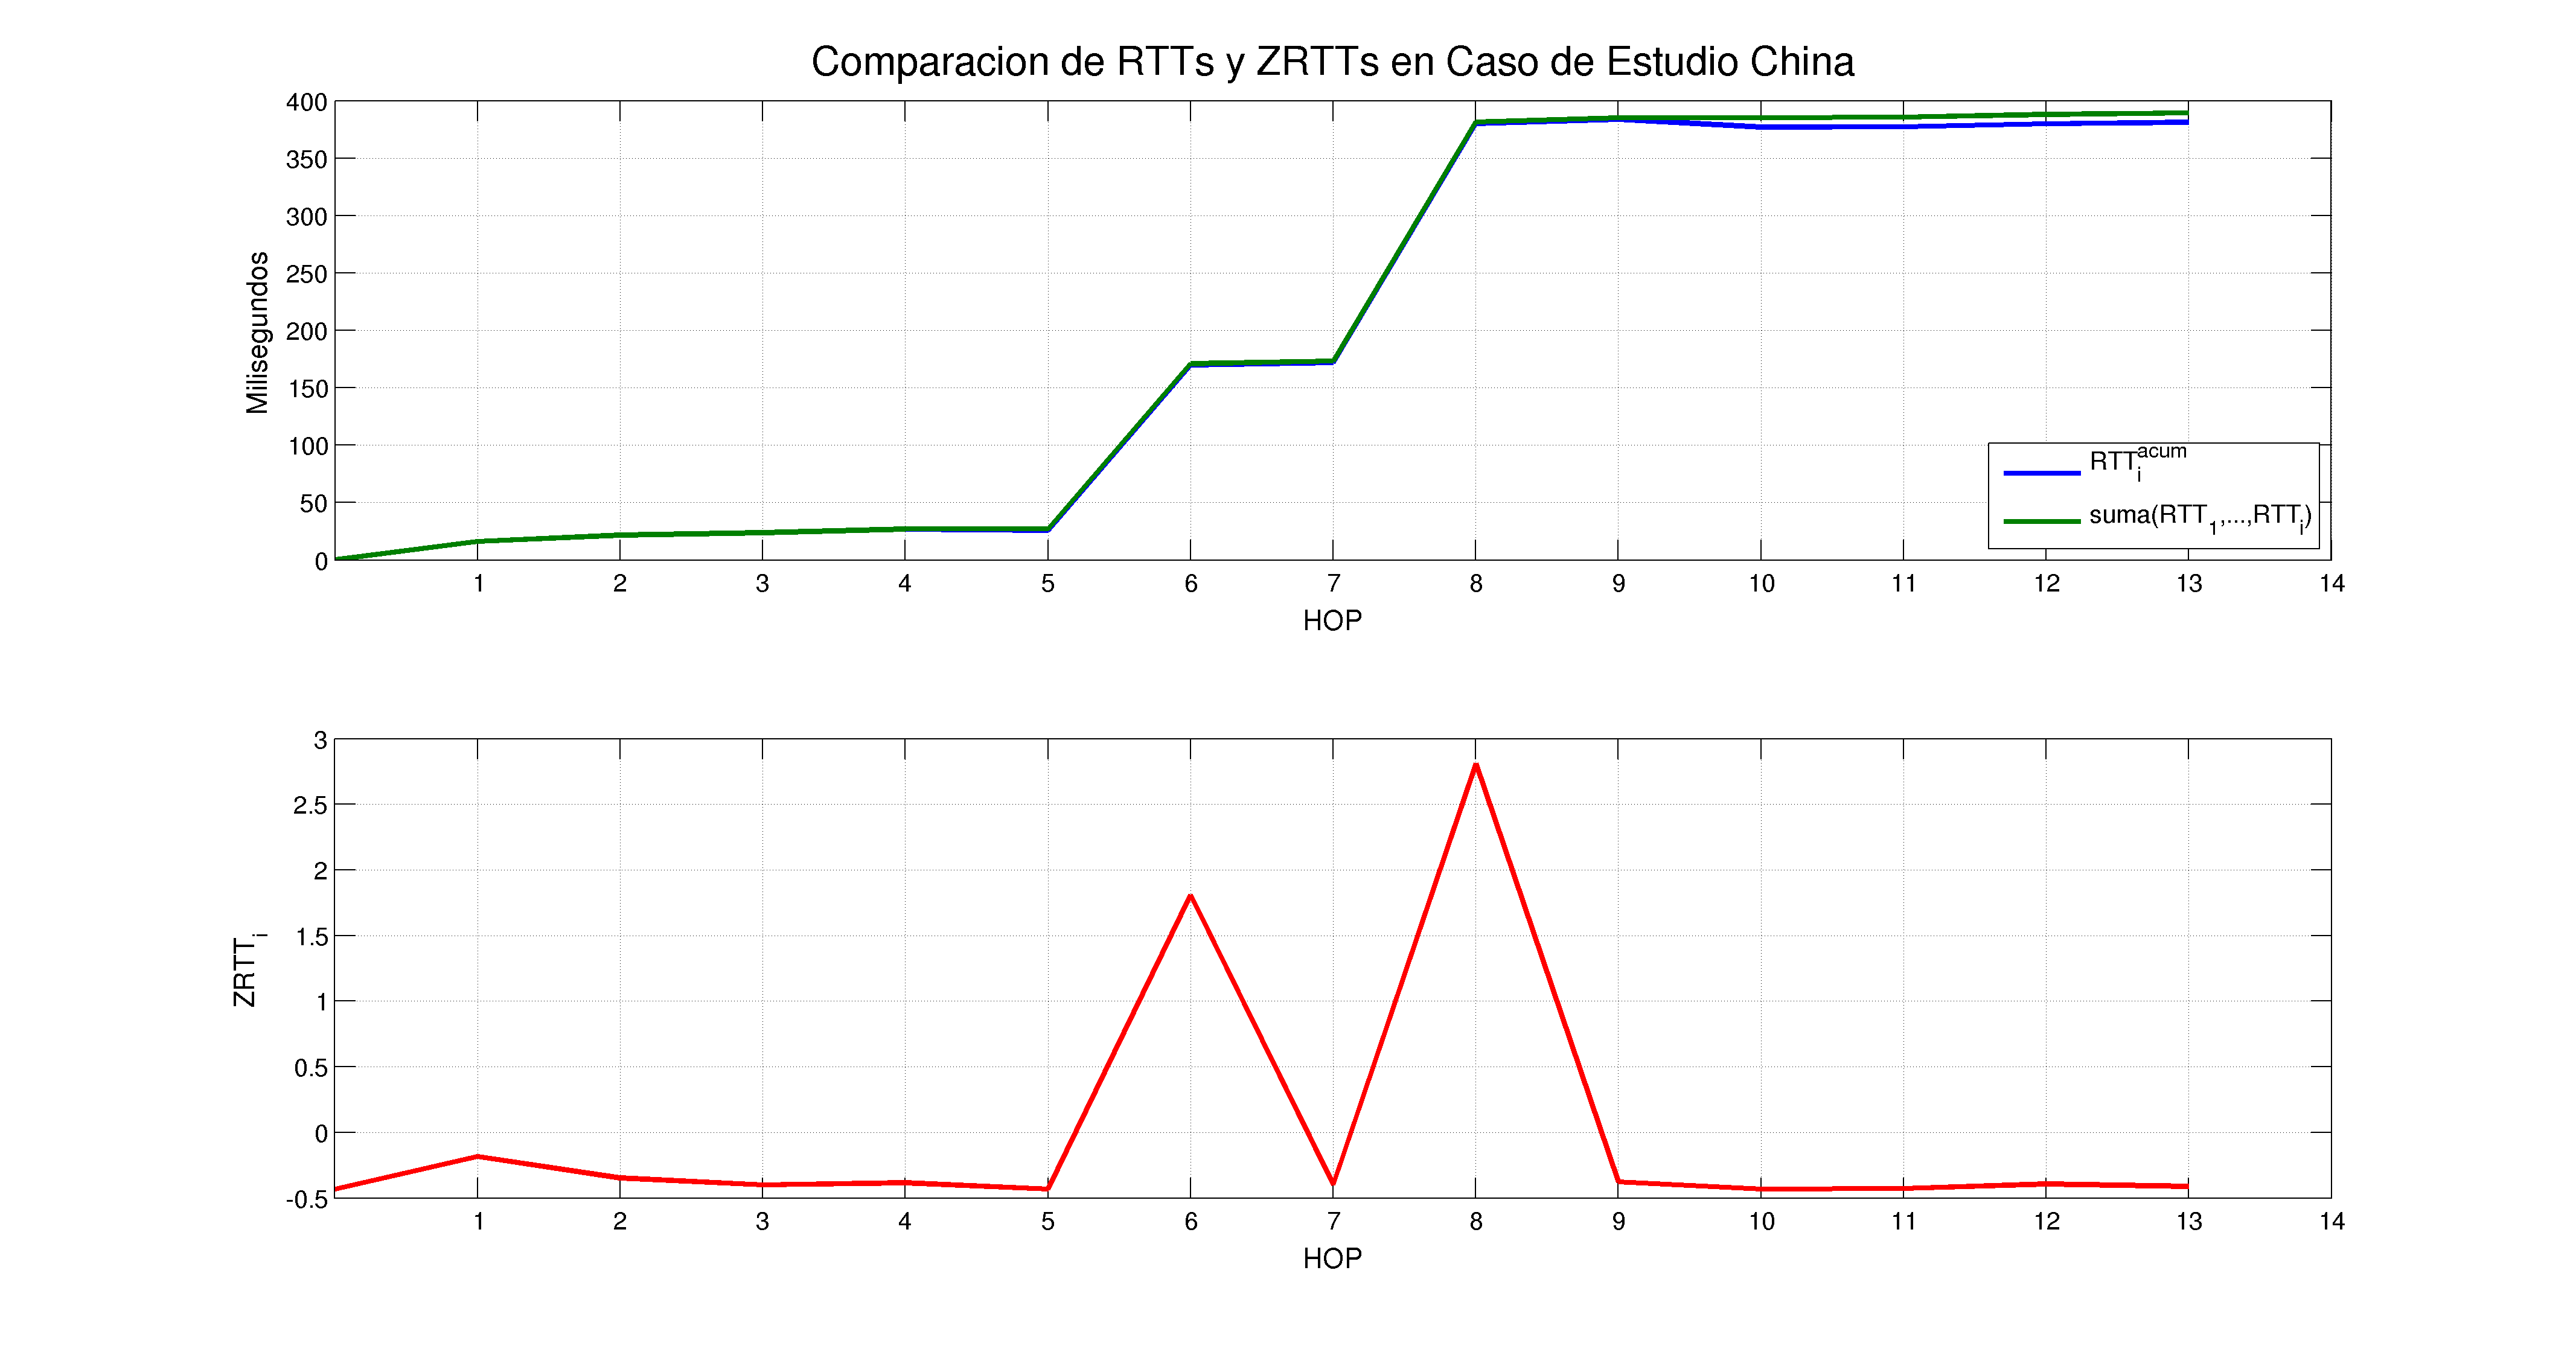
\includegraphics[width=\textwidth]{../resultados/comparacion-zrtts-china.png}
 \caption{Comparación de $RTT^{acum}_i$ con $\sum_{k=1}^{i}RTT_k$ y con $ZRTT_i$.}
 \label{resultados:china:zrtt}
\end{figure}


\newpage
\subsubsection{Geolocalización}

\begin{table}[h!]
  \centering
  \scriptsize
  \begin{adjustwidth}{-0.5cm}{}
    \begin{tabular}{| r | r | c | c | c |}
    \hline
    \multicolumn{5}{|c|}{\bf Geolocalización: China}\\
    \hline\hline
    {\bf TTL} & \multicolumn{1}{|c|}{\bf IP} & \multicolumn{1}{|c|}{\bf DNS} & {\bf Ubicación} & {\bf Lat,Lon}\\
    \hline
    \hline
    %%%% TABLA QUE PRODUCE calcular.py :
    \input{../resultados/geoloc-china.tab}
    \end{tabular}
  \end{adjustwidth}
  \caption{\footnotesize Tabla de información de geolocalización del camino más probable para el caso de estudio China. Observar las celdas resaltadas de arriba hacia abajo: (1) indica que comenzamos en Argentina. (2) dice ``{\tt crossing-argentina}'' lo cual indica que seguimos en Argentina o  cerca. (3) dice ``{\tt ar4.LAX1}'' mientras que las dos anteriores decían ``{\tt ar3.eze1}'' indicando que algo cambió, la red también cambió (ver la IP) y además este salto corresponde al de mayor RTT. (4) Este es el segundo salto de mayor RTT, observar que dice ``{\tt hkg05}'', lo cual se puede interpretar
  como una sigla para ``Hong Kong'', además es razonable creer esto porque todos los saltos restantes tienen ubicación en esa ciudad.}
\end{table}

\begin{figure}[h!]
 \centering
 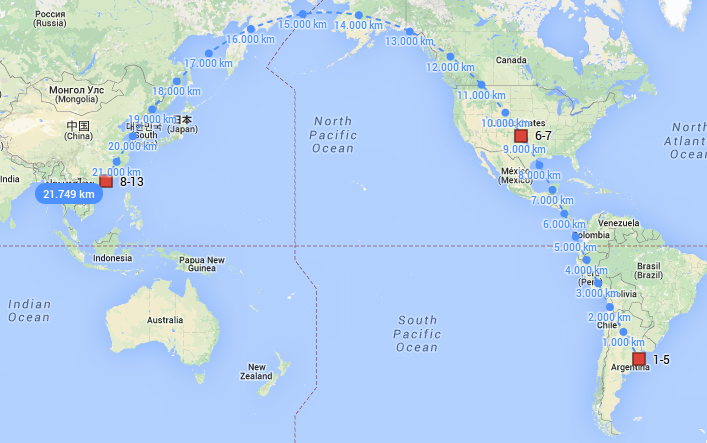
\includegraphics[width=\textwidth]{../resultados/mapa-china.png}
 \caption{Mapa generado utilizando los datos de la tabla anterior y los valores de $RRT_i$ empíricos.}
\end{figure}
% Mapa geolocalizando la ruta
% distancias vs rtts, acertamos al enlace submarino con los zscores?

\newpage
